\thispagestyle{empty}
\section{\textbf{\Large{Задание :}}}
По выданному преподавателем варианту восстановить текст заданного варианта программы, определить предназначение и составить описание программы, определить область представления и область допустимых значений исходных данных и результата, выполнить трассировку программы.
\begin{center}
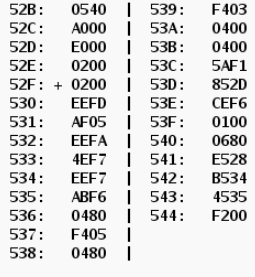
\includegraphics{img/Task.PNG}
\end{center}
\section{\textbf{\Large{Программа :}}}
\begin{center}
\begin{tabular}{|c|c|c|l|}
\hline
\textbf{Адрес ячейки} & \textbf{Содержимое ячейки} & \textbf{Мнемоника} & \textbf{Комментарии} \\
\hline
52B & 0540 & --- & Адрес начала массива \\
\hline
52C	& A000 & --- & Ячейка для хранения адреса \\
 & & & обрабатываемого элемента массива \\
\hline
52D	& E000 & --- & Ячейка для хранения количества \\
 & & &необработанных элементов массива \\
\hline
52E	& 0200 & --- & Ячейка для записи результата  \\ 
& & & работы программы \\
\hline
52F & +0200 & CLA & Очистка аккумулятора \\
\hline
530	& EEFD & ST (IP - 3) &  Сохранение в 0x52E \\
\hline
531 & AF05 & LD \#0x5 & Загружаем в AC 0x5 (Длина массива) \\
\hline
532 & EEFA & ST (IP - 6) & Сохранение в 0x52D \\
\hline
533 & 4EF7 & ADD (IP - 9) & Логическое сложение из 0x52B \\
\hline
534	& EEF7 & ST (IP - 9) & Сохранение в 0x52C \\
\hline
535 & ABF6 & LD –(IP - 10) & Загружаем элемент массива в 0x52C\\
& & &  (предекремент) \\
536 & 0480 & ROR & Циклический сдвиг вправо  \\
537	& F405 & BLO 05 & IF C==1 THEN IP$\rightarrow$53D \\
538 & 0480 & ROR & Циклический сдвиг вправо  \\
539	& F405 & BLO 03 & IF C==1 THEN IP$\rightarrow$53D \\
53A & 0400 & ROL & Циклический сдвиг влево \\
53B & 0400 & ROL & Циклический сдвиг влево \\
53C & 5AF1 & ADC (IP-15)+ &  Сложение с переносом AC, \\
& & & MEM(0x52E)+1$\rightarrow$MEM(0x52E)\\
53D & 852D & LOOP 52D & MEM(0x52D)-1$\rightarrow$ MEM(0x52D) \\
& & & IF MEM(0x52D)$\leq$0 THEN IP+1$\rightarrow$IP \\
53E & CEF6 & BR  IP - 10 & Безусловный переход в 0x535 \\
53F & 0200 & HLT & Останов \\
\hline 
540 & 0680 & & \\
541	& E528 & & \\
542	& B534 & & Элементы массива \\
543	& 4535 & & \\
544	& F200 & & \\
\hline
\end{tabular}
\end{center}
\newpage
\thispagestyle{empty}
\section{\textbf{\Large{Описание программы :}}}
\subsection{Назначение программы :}
Программа просматривает каждый элемент в массиве, если есть делитель на четыре, результат увеличивается на единицу
\[MEM(0x52E) =  \sum_{n=1}^{5} 1 *
\begin{cases}
    1       & \text{if } a[i] \text{ mod 4 = 0} \\
    0       & \text{if } a[i]  \text{ mod 4 != 0}
\end{cases}
\]
\subsection{Область представления и область допустимых значений исходных данных и результата :}
\subsubsection{Область представления :}
52C-52E,540-544: 16-разрядные знаковые целые числа,.\\
Диапазон значений формата: $-2^{15}\ldots2^{15}-1$ \\
52B: 11-разрядное беззнаковое целое число. \\
Диапазон значений формата: $0\ldots2^{11} - 1$
\subsubsection{Область допустимых значений :}
52C-52E,540-544 : [-32768; 32767]; \\
58B : $[000, 526]\cup[540,7FF]$ \\
\subsection{Расположение в памяти программы, исходных данных и результатов :}
B (0x52B) : aдрес начала массива \\
R (0x52E) : ячейка для записи результата работы программы \\
Ячейки 52C, 52D : вспомогательные ячейки для хранения данных, нужных для функционирования программы\\
Ячейки 52F-53F : код программы \\
\subsection{Адреса первой и последней выполняемой команд программы :}
Ячейка 52F : первая исполняемая команда\\
Ячейка 53F : последняя исполняемая команда\\
\newpage
\section{\textbf{\Large{Трассировка :}}}
\thispagestyle{empty}
\begin{center}
	\begin{tabular}{|c|c|c|c|c|c|c|c|c|c|c|c|}
		\hline
		\multicolumn{2}{|c}{\makecell{\textbf{Выполняемая}\\\textbf{команда}}}
		&\multicolumn{8}{|c|}{\textbf{Содердимое регистров после выполнения команды}}
		&\multicolumn{2}{c|}{\makecell{\textbf{Ячейка, содержимое}\\\textbf{которой изменилось}}}\\
		\hline
		Адрес & Код & IP & CR & AR & DR & SP & BR & AC & NZVC & Адрес & Новый код\\
		\hline
        52F & 0200  & 530	& 0200	& 52F	& 0200	& 000	& 052F	& 0000	& 0100 & &  \\
        \hline
        530	& EEFD	& 531	& EEFD	& 52E	& 0000	& 000	& FFFD	& 0000	& 0100	& 52E	& 0000 \\
        \hline
        531	& AF05	& 532	& AF05	& 531	& 0005	& 000	& 0005	& 0005	& 0000 & & \\
        \hline
        532	& EEFA	& 533	& EEFA	& 52D	& 0005	& 000	& FFFA	& 0005	& 0000	& 52D	& 0005 \\
        \hline
        533	& 4EF7	& 534	& 4EF7	& 52B	& 0540	& 000	& FFF7	& 0545	& 0000 & & \\
        \hline
        534	& EEF7	& 535	& EEF7	& 52C	& 0545	& 000	& FFF7	& 0545	& 0000	& 52C	& 0545 \\
        \hline
        535	& ABF6	& 536	& ABF6	& 544	& F200	& 000	& FFF6	& F200	& 1000	& 52C	& 0544 \\
        \hline
        536	& 0480	& 537	& 0480	& 536	& 0480	& 000	& 0536	& 7900	& 0000 & & \\
        \hline
        537	& F405	& 538	& F405	& 537	& F405	& 000	& 0537	& 7900  & 0000 & & \\
        \hline
        538	& 0480	& 539	& 0480	& 538	& 0480	& 000	& 0538	& 3C80	& 0000 & & \\
        \hline
        539	& F403	& 53A	& F403	& 539	& F403	& 000	& 0539	& 3C80	& 0000 & & \\
        \hline
        53A	& 0400	& 53B	& 0400	& 53A	& 0400	& 000	& 053A	& 7900	& 0000 & & \\
        \hline
        53B	& 0400	& 53C	& 0400	& 53B	& 0400	& 000	& 053B	& F200	& 1010 & & \\
        \hline
        53C	& 5AF1	& 53D	& 5AF1	& 000	& 0000	& 000	& FFF1	& F200	& 1000	& 52E	& 0001 \\
        \hline
        53D	& 852D	& 53E	& 852D	& 52D	& 0004	& 000	& 0003	& F200	& 1000	& 52D	& 0004 \\
        \hline
        53E	& CEF6	& 535	& CEF6	& 53E	& 0535	& 000	& FFF6	& F200	& 1000 & & \\
        \hline
        535	& ABF6	& 536	& ABF6	& 543	& 4535	& 000	& FFF6	& 4535	& 0000	& 52C	& 0543 \\
        \hline
        536	& 0480	& 537	& 0480	& 536	& 0480	& 000	& 0536	& 229A	& 0011 & & \\
        \hline
        537	& F405	& 53D	& F405	& 537	& F405	& 000	& 0005	& 229A	& 0011 & & \\
        \hline
        53D	& 852D	& 53E	& 852D	& 52D	& 0003	& 000	& 0002	& 229A	& 0011	& 52D	& 0003 \\
        \hline
        53E	& CEF6	& 535	& CEF6	& 53E	& 0535	& 000	& FFF6	& 229A	& 0011 & & \\
        \hline
        535	& ABF6	& 536	& ABF6	& 542	& B534	& 000	& FFF6	& B534	& 1001	& 52C	& 0542 \\
        \hline
        536	& 0480	& 537	& 0480	& 536	& 0480	& 000	& 0536	& DA9A	& 1010 & & \\
        \hline
        537	& F405	& 538	& F405	& 537	& F405	& 000	& 0537	& DA9A	& 1010 & & \\
        \hline
        538	& 0480	& 539	& 0480	& 538	& 0480	& 000	& 0538	& 6D4D	& 0000 & & \\
        \hline
        539	& F403	& 53A	& F403	& 539	& F403	& 000	& 0539	& 6D4D	& 0000 & & \\
        \hline
        53A	& 0400	& 53B	& 0400	& 53A	& 0400	& 000	& 053A	& DA9A	& 1010 & & \\
        \hline
        53B	& 0400	& 53C	& 0400	& 53B	& 0400	& 000	& 053B	& B534	& 1001 & & \\
        \hline
        53C	& 5AF1	& 53D	& 5AF1	& 001	& 0000	& 000	& FFF1	& B535	& 1000	& 52E	& 0002 \\
        \hline
        53D	& 852D	& 53E	& 852D	& 52D	& 0002	& 000	& 0001	& B535	& 1000	& 52D	& 0002 \\
        \hline
        53E	& CEF6	& 535	& CEF6	& 53E	& 0535	& 000	& FFF6	& B535	& 1000 & & \\
        \hline
        535	& ABF6	& 536	& ABF6	& 541	& E528	& 000	& FFF6	& E528	& 1000	& 52C	& 0541 \\
        \hline
        536	& 0480	& 537	& 0480	& 536	& 0480	& 000	& 0536	& 7294	& 0000 & & \\
        \hline
        537	& F405	& 538	& F405	& 537	& F405	& 000	& 0537	& 7294	& 0000 & & \\
        \hline
        538	& 0480	& 539	& 0480	& 538	& 0480	& 000	& 0538	& 394A	& 0000 & & \\
        \hline
        539	& F403	& 53A	& F403	& 539	& F403	& 000	& 0539	& 394A	& 0000 & & \\
        \hline
        53A	& 0400	& 53B	& 0400	& 53A	& 0400	& 000	& 053A	& 7294	& 0000 & & \\
        \hline
        53B	& 0400	& 53C	& 0400	& 53B 	& 0400	& 000	& 053B	& E528	& 1010 & & \\
        \hline
        53C	& 5AF1	& 53D	& 5AF1	& 002	& 0000	& 000	& FFF1	& E528	& 1000  & 52E	& 0003 \\
        \hline
        53D	& 852D	& 53E	& 852D	& 52D	& 0001	& 000	& 0000	& E528	& 1000  & 52D	& 0001 \\
        \hline
        53E	& CEF6	& 535	& CEF6	& 53E	& 0535	& 000	& FFF6	& E528	& 1000 & & \\
        \hline
        535	& ABF6	& 536	& ABF6	& 540	& 0680	& 000	& FFF6	& 0680	& 0000	& 52C	& 0540 \\
        \hline
        536	& 0480	& 537	& 0480	& 536	& 0480	& 000	& 0536	& 0340	& 0000 & & \\
        \hline
        537	& F405	& 538	& F405	& 537	& F405	& 000	& 0537	& 0340	& 0000 & & \\
        \hline
        538	& 0480	& 539	& 0480	& 538	& 0480	& 000	& 0538	& 01A0	& 0000 & & \\
        \hline
        539	& F403	& 53A	& F403	& 539	& F403	& 000	& 0539	& 01A0	& 0000 & & \\
        \hline
        53A	& 0400	& 53B	& 0400	& 53A	& 0400	& 000	& 053A	& 0340	& 0000 & & \\
        \hline
        53B	& 0400	& 53C	& 0400	& 53B	& 0400	& 000	& 053B	& 0680	& 0000 & & \\
        \hline
        53C	& 5AF1	& 53D	& 5AF1	& 003	& 0000	& 000	& FFF1	& 0680	& 0000	& 52E	& 0004 \\
        \hline
        53D	& 852D	& 53F	& 852D	& 52D	& 0000	& 000	& FFFF	& 0680	& 0000	& 52D	& 0000 \\
        \hline
        53F	& 0100	& 540	& 0100	& 53F	& 0100	& 000	& 053F	& 0680	& 0000 & & \\
        \hline
	\end{tabular}
\end{center}
\newpage
\thispagestyle{empty}
\section{\textbf{\Large{Вывод :}}}
В ходе лабораторных работ я узнал способ организации циклических программ в БЭВМ. Режимы адресации и как это работает в БЭВМ.